% Presentación para el foro (máximo 4 diapositivas) — Grupo 2, Auditoría o Control
% Mismo formato que la presentación final de Estadística (Madrid, color vino).
% Compilar con pdfLaTeX (compilador por defecto de Overleaf).
\documentclass{beamer}
\usetheme{Madrid}
\usepackage[utf8]{inputenc}
\usepackage[provide=*,spanish]{babel}
\usepackage{amsmath,amssymb}
\usepackage{booktabs}
\usepackage{pgfplots}
\pgfplotsset{compat=1.17,
  leyenda linea/.style={legend image code/.code={\draw[##1] (0cm,0cm) -- (0.45cm,0cm);}}}

% ---------------- Colores y fuentes del formato ----------------
\definecolor{vino}{RGB}{80,0,0}
\definecolor{vinoclaro}{RGB}{160,90,90}
\usecolortheme[named=vino]{structure}
\setbeamercolor{palette primary}{bg=vino,fg=white}
\setbeamercolor{palette secondary}{bg=vino,fg=white}
\setbeamercolor{palette tertiary}{bg=vino!50!black,fg=white}
\setbeamercolor{frametitle}{bg=vino,fg=white}
\setbeamercolor{title}{bg=vino,fg=white}
\setbeamercolor{author in head/foot}{bg=vino!50!black,fg=white}
\setbeamercolor{title in head/foot}{bg=vino,fg=white}
\setbeamercolor{date in head/foot}{bg=vino,fg=white}
\setbeamercolor{block title}{bg=vino,fg=white}
\setbeamercolor{block body}{bg=vino!8}
\setbeamerfont{frametitle}{family=\rmfamily,size=\Large}
\setbeamerfont{title}{family=\rmfamily,series=\bfseries}
\setbeamerfont{footline}{family=\rmfamily}
\setbeamerfont{block title}{family=\rmfamily,series=\bfseries,size=\small}
\setbeamertemplate{caption}[numbered]
\setbeamercolor{caption name}{fg=vino}
\setbeamerfont{caption name}{family=\rmfamily,series=\bfseries}
\setbeamerfont{caption}{size=\scriptsize}
\setbeamercolor{normal text}{fg=black}
\setbeamercolor{alerted text}{fg=black}
\AtBeginDocument{\renewcommand{\tablename}{Tabla}\renewcommand{\figurename}{Figura}}
\newcommand{\nota}[1]{\par\vspace{2pt}{\scriptsize\textit{Nota.} #1}\par}

% ---------------- Datos de la portada y del pie ----------------
\title[Proyecto Final]{Seguro colectivo de fallecimiento y cuenta equity-linked: robustez ante mayor renuncia}
\author[Andrey, Anthonny, Randal]{Andrey González Bastos (C33329)\\Randal Picado Bermúdez (C36024)\\Anthonny Flores Rojas (C32975)}
\date[]{Grupo 2, Auditoría o Control \,|\, CA-0309}

\begin{document}

% La guía permite máximo cuatro diapositivas, por eso no se incluye portada.
% Si la profesora no cuenta la portada, descomenten la siguiente línea:
% \begin{frame}\titlepage\end{frame}

% =================================================================
\begin{frame}{Escenario único del grupo 2}
\small
\begin{itemize}
\item Prima anual de 55\,000 y renuncia anual de decremento único del 6\,\%.
\item Se mantienen rendimiento del 5\,\%, gasto de 10\,000, descuento del 4\,\% y el cuadro de reservas.
\item Estrés académico, no la reacción estimada de los afiliados. Se compara con la base de C.
\end{itemize}
\vspace{-4pt}

\begin{table}
\caption{Caso base frente al escenario del grupo 2}
\scriptsize
\begin{tabular}{lrr}
\toprule
Indicador & Base & Prima 55\,000 y renuncia 6\,\%\\
\midrule
Activos al cierre del año 5 & 84\,700.19 & 72\,387.73\\
NPV (millones de u.m.) & $-12\,912.86$ & $-10\,222.77$\\
Margen sobre primas descontadas & $-57.88\,\%$ & $-44.09\,\%$\\
Total de aportes (millones de u.m.) & 3\,050.20 & 0.00\\
$\tilde F_1 - V_1$ (millones de u.m.) & $-2\,024.61$ & $-1\,307.79$\\
\bottomrule
\end{tabular}
\end{table}
\nota{El NPV mejora porque hay 12\,312 asegurados menos, no porque el producto deje de perder.}
\end{frame}

% =================================================================
\begin{frame}{Resultados: la tarifa no cubre el siniestro esperado}
\begin{columns}[T]
\begin{column}{0.56\textwidth}
\begin{figure}
\caption{Siniestro esperado y prima neta por contrato}
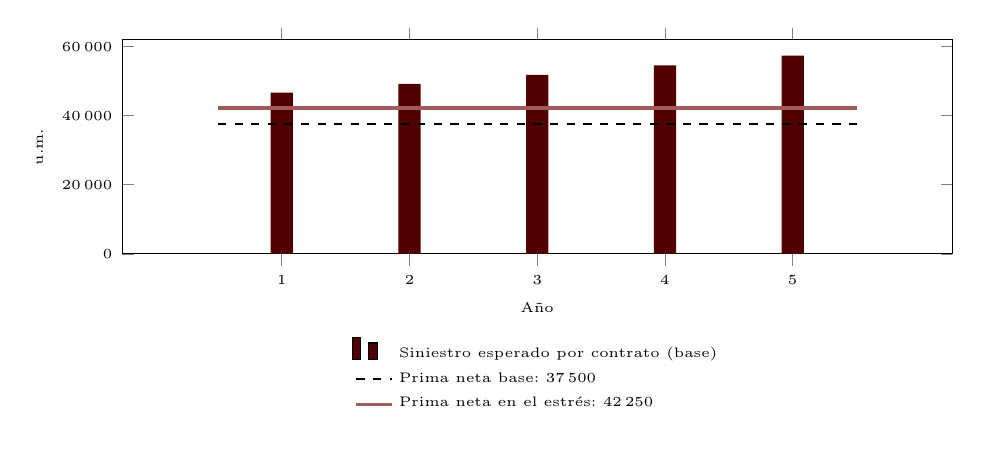
\begin{tikzpicture}
\begin{axis}[
  width=\linewidth, height=4.3cm,
  ybar, bar width=8pt, ymin=0, ymax=62000,
  xtick={1,2,3,4,5}, xlabel={Año}, ylabel={u.m.},
  label style={font=\tiny}, tick label style={font=\tiny},
  scaled y ticks=false,
  yticklabel style={/pgf/number format/.cd,1000 sep={\,}},
  legend style={font=\tiny,at={(0.5,-0.36)},anchor=north,draw=none,legend columns=1},
  legend cell align=left, enlarge x limits=0.15]
\addplot[fill=vino,draw=none] coordinates {(1,46659) (2,49224) (3,51865) (4,54589) (5,57392)};
\addlegendentry{Siniestro esperado por contrato (base)}
\addplot[sharp plot,black,thick,dashed,mark=none,leyenda linea] coordinates {(0.5,37500) (5.5,37500)};
\addlegendentry{Prima neta base: 37\,500}
\addplot[sharp plot,vinoclaro,very thick,mark=none,leyenda linea] coordinates {(0.5,42250) (5.5,42250)};
\addlegendentry{Prima neta en el estrés: 42\,250}
\end{axis}
\end{tikzpicture}
\end{figure}
\end{column}
\begin{column}{0.42\textwidth}
\footnotesize
\begin{itemize}
\item NPV base: $-12\,912.86$ millones; margen de $-57.88\,\%$.
\item La adquisición explica 7\,800.30 millones (60\,\%).
\item El faltante existe desde el año 1 y crece con la edad de la cartera.
\item Adverso: NPV de $-13\,617.35$ millones.
\end{itemize}
\end{column}
\end{columns}
\nota{Prima neta = prima menos gasto y comisión. Siniestro = $5\,000\,000 \times$ probabilidad de muerte por contrato vigente.}
\end{frame}

% =================================================================
\begin{frame}{Resultados: los recursos no respaldan la reserva}
\begin{columns}[T]
\begin{column}{0.52\textwidth}
\begin{figure}
\caption{Recursos menos reserva al cierre del año 1}
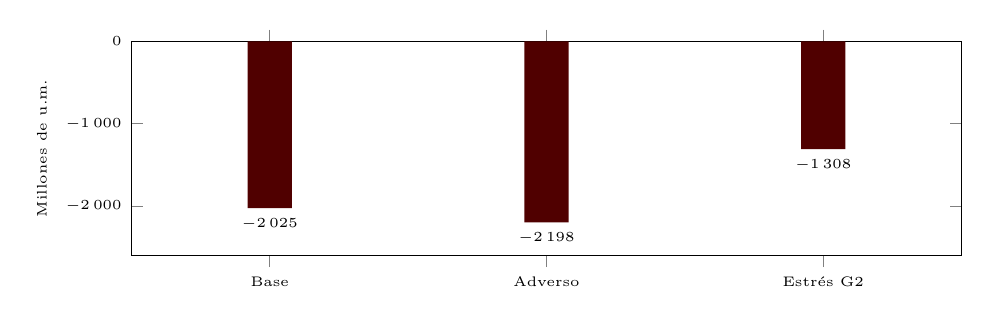
\begin{tikzpicture}
\begin{axis}[
  width=\linewidth, height=4.3cm,
  ybar, bar width=16pt, ymin=-2600, ymax=0,
  symbolic x coords={Base,Adverso,Estrés G2}, xtick=data,
  ylabel={Millones de u.m.},
  label style={font=\tiny}, tick label style={font=\tiny},
  scaled y ticks=false,
  yticklabel style={/pgf/number format/.cd,1000 sep={\,}},
  nodes near coords, nodes near coords style={font=\tiny,anchor=north},
  every node near coord/.append style={/pgf/number format/.cd,fixed,precision=0,1000 sep={\,}},
  enlarge x limits=0.25]
\addplot[fill=vino,draw=none] coordinates {(Base,-2024.61) (Adverso,-2197.78) (Estrés G2,-1307.79)};
\end{axis}
\end{tikzpicture}
\end{figure}
\end{column}
\begin{column}{0.46\textwidth}
\footnotesize
\begin{itemize}
\item $\tilde F_1 - V_1 < 0$ en los tres escenarios.
\item Recursos de 25\,000 por contrato contra una reserva de 40\,000.
\item Aportes: 3\,050.20 millones (base) y 3\,807.06 (adverso).
\item El estrés elimina los aportes, pero el respaldo sigue negativo del año 1 al 4.
\end{itemize}
\end{column}
\end{columns}
\nota{$\tilde F_1$ es el saldo de recursos antes del aporte del año 1 y $V_1$ la reserva total suministrada al cierre.}
\end{frame}

% =================================================================
\begin{frame}{Resultados: cuenta equity-linked y opinión}
\begin{table}
\caption{Comparación de garantías con las mismas 1\,000 trayectorias (u.m.)}
\scriptsize
\begin{tabular}{lrr}
\toprule
Indicador & $G = 100\,000$ & $G = 110\,000$\\
\midrule
VP medio del complemento & 5\,126.70 & 8\,087.64\\
NPV medio del proveedor & 4\,054.40 & 1\,093.45\\
Frecuencia de activación de la garantía & 36.7\,\% & 48.5\,\%\\
Frecuencia de pérdida (NPV $< 0$) & 24.6\,\% & 33.9\,\%\\
CTE95 (media de las 50 mayores pérdidas) & 22\,959.79 & 29\,892.45\\
\bottomrule
\end{tabular}
\end{table}
\nota{R, Mersenne-Twister, semilla 2026. La garantía mayor nunca aumenta el NPV de ninguna trayectoria.}

\vspace{4pt}
\begin{block}{Opinión preliminar del grupo 2}
\footnotesize
\textbf{Posponer} el seguro colectivo hasta tener NPV $\ge 0$ en base y adverso y un plan de
capital que respalde la reserva desde el año 1. \textbf{Apoyar} la cuenta con $G = 100\,000$,
condicionada a monitorear la cola de pérdidas.
\end{block}
\end{frame}

\end{document}
